\documentclass[tikz,border=5pt]{standalone}
\usepackage{pgfplots}
\usepgfplotslibrary{groupplots}
\pgfplotsset{compat=1.18}

\definecolor{corba}{HTML}{365FB3}
\definecolor{punt}{HTML}{B91C1C}
\definecolor{assimptota}{HTML}{6B7280}

\begin{document}
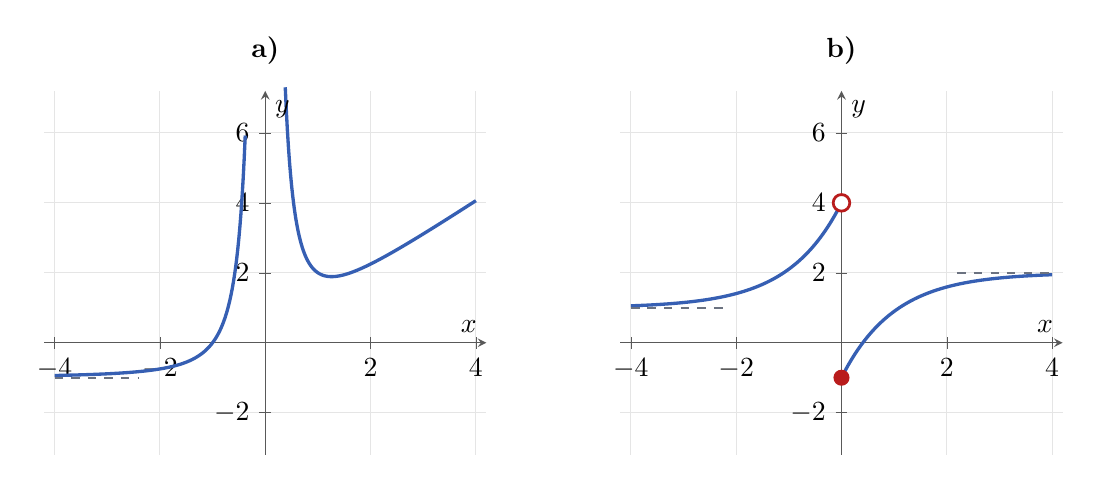
\begin{tikzpicture}
  \begin{groupplot}[
    group style={group size=2 by 1, horizontal sep=1.7cm},
    width=7.2cm,
    height=6.2cm,
    axis lines=middle,
    xmin=-4.2,
    xmax=4.2,
    ymin=-3.2,
    ymax=7.2,
    xlabel={$x$},
    ylabel={$y$},
    xtick={-4,-2,0,2,4},
    ytick={-2,0,2,4,6},
    grid=major,
    grid style={black!10},
    axis line style={black!65},
    tick style={black!65},
    clip=false,
  ]
    \nextgroupplot[title={\textbf{a)}}]
      \addplot[corba, very thick, domain=-4:-0.38, samples=180]
        {-1+1/(x^2)};
      \addplot[corba, very thick, domain=0.38:4, samples=180]
        {x+1/(x^2)};
      \addplot[assimptota, dashed, thick, domain=-4:-2.4] {-1};

    \nextgroupplot[title={\textbf{b)}}]
      \addplot[corba, very thick, domain=-4:0, samples=160]
        {1+3*exp(x)};
      \addplot[corba, very thick, domain=0:4, samples=160]
        {2-3*exp(-x)};
      \addplot[assimptota, dashed, thick, domain=-4:-2.2] {1};
      \addplot[assimptota, dashed, thick, domain=2.2:4] {2};
      \addplot[
        only marks,
        mark=*,
        mark size=3pt,
        mark options={draw=punt, fill=white, line width=1pt}
      ] coordinates {(0,4)};
      \addplot[
        only marks,
        mark=*,
        mark size=2.7pt,
        mark options={draw=punt, fill=punt}
      ] coordinates {(0,-1)};
  \end{groupplot}
\end{tikzpicture}
\end{document}
